\documentclass[tikz,border=12pt]{standalone}
\usepackage{circuitikz}
\usepackage{xcolor}
\usepackage{amsmath}
\usepackage{amssymb}
\usetikzlibrary{arrows.meta, positioning, decorations.pathreplacing, calc, fit, backgrounds}

\begin{document}
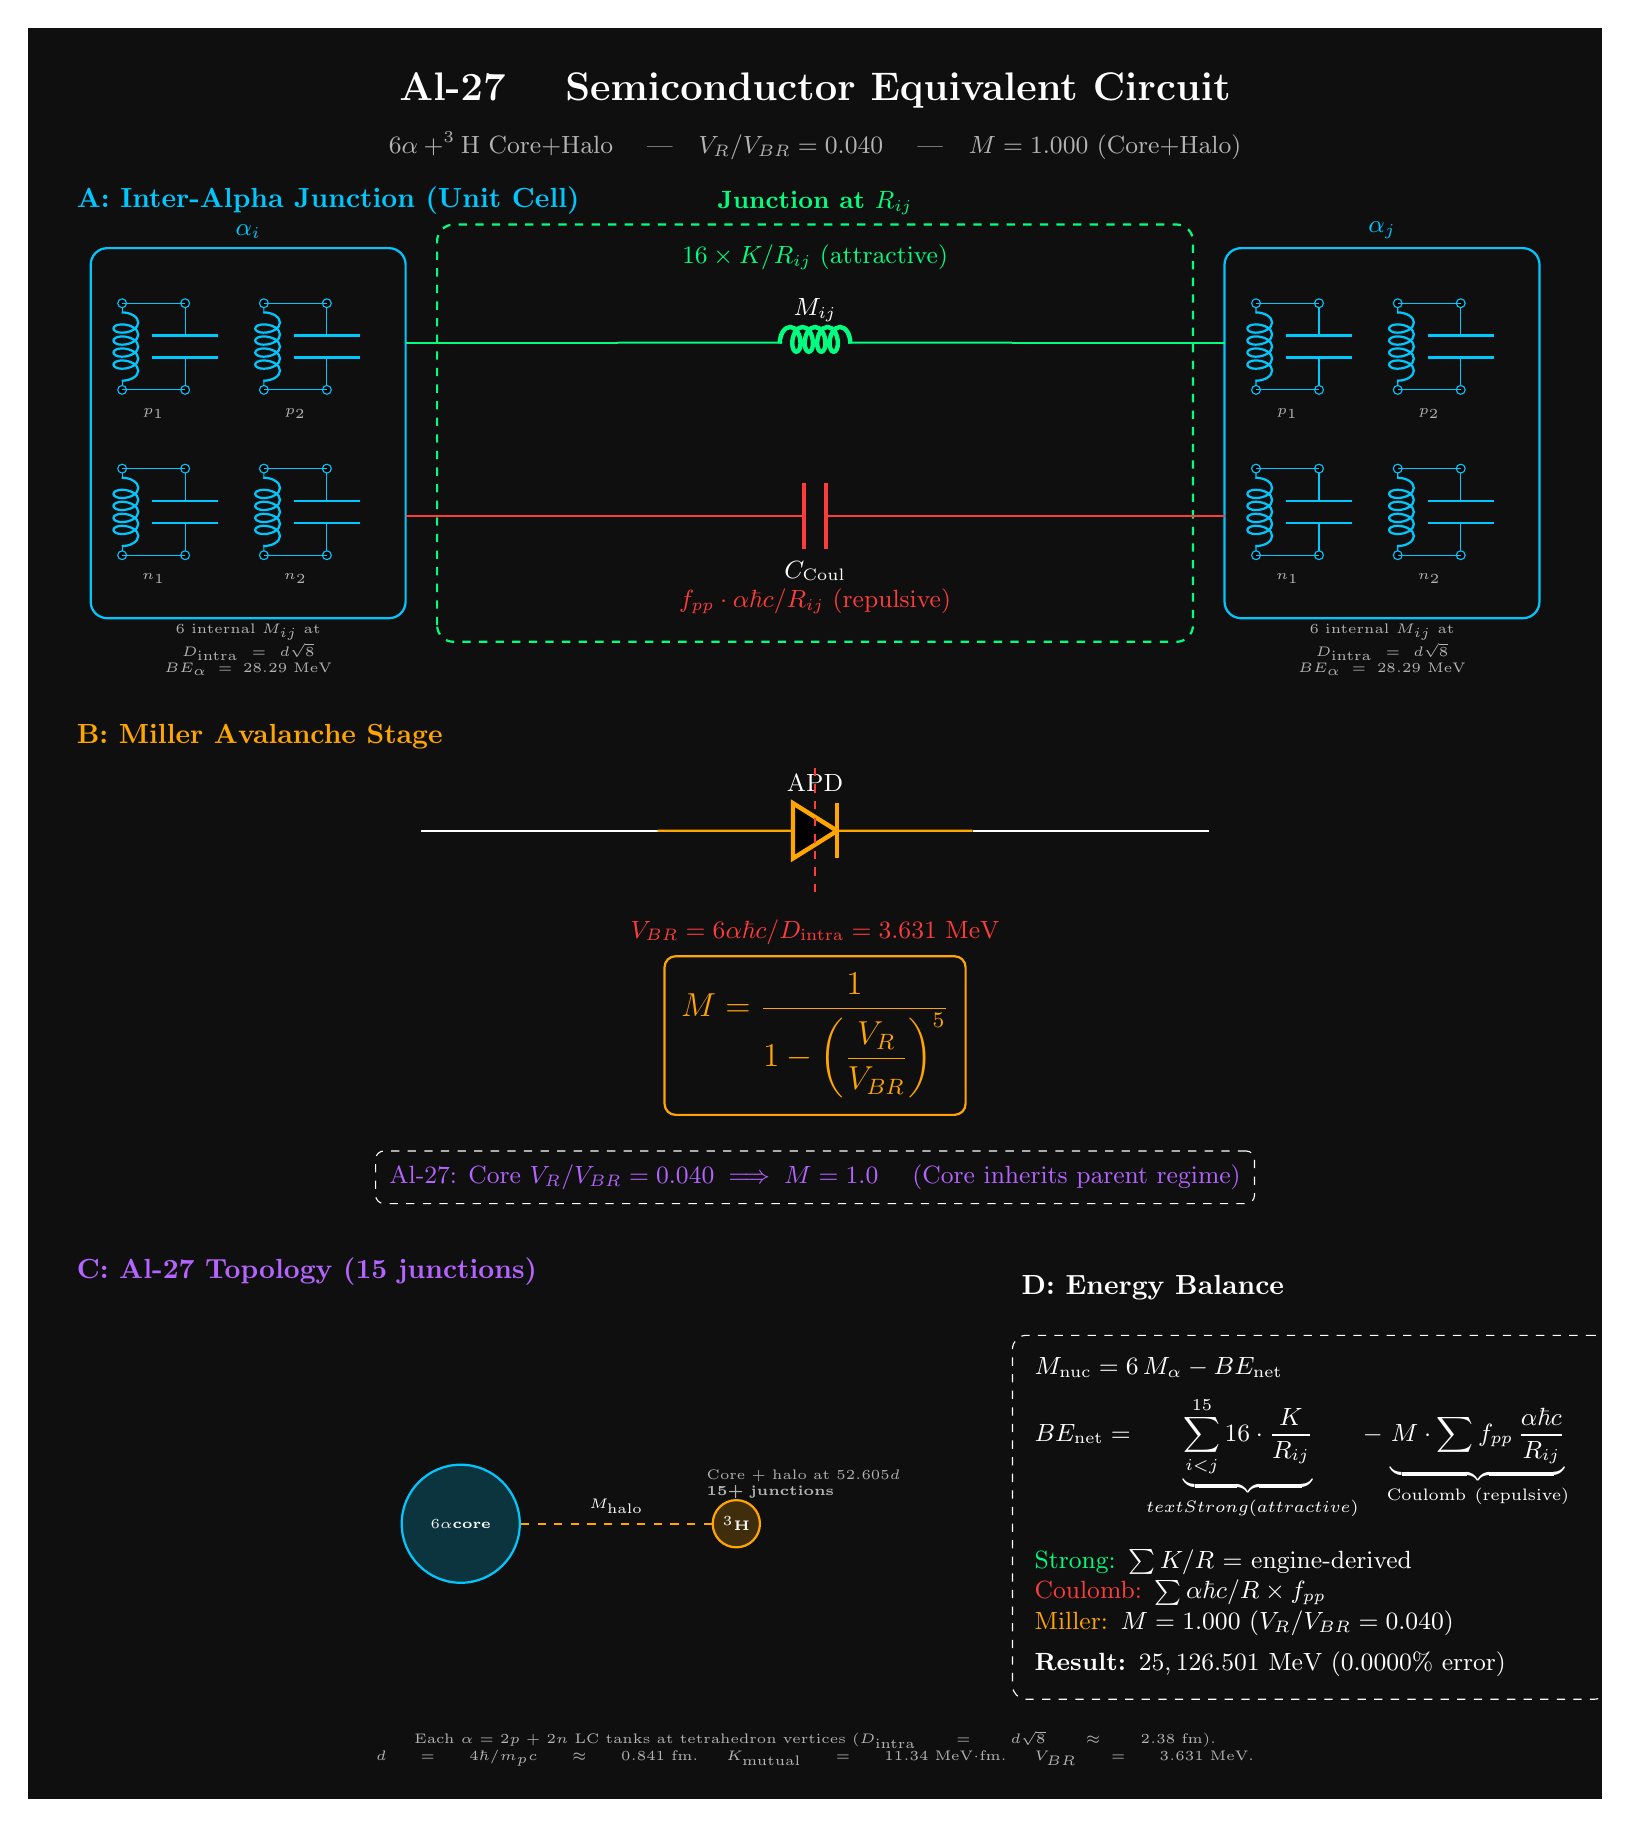
\begin{tikzpicture}[>=latex, font=\small]

\definecolor{darkbg}{RGB}{15, 15, 15}
\definecolor{neonblue}{RGB}{0, 200, 255}
\definecolor{neongreen}{RGB}{0, 255, 128}
\definecolor{neonorange}{RGB}{255, 165, 0}
\definecolor{neonred}{RGB}{255, 60, 60}
\definecolor{neonpurple}{RGB}{180, 100, 255}
\definecolor{dimwhite}{RGB}{180, 180, 180}

% Background
\fill[darkbg] (-10,-13.5) rectangle (10,9);

% TITLE
\node[text=white, font=\bfseries\Large] at (0, 8.2)
    {Al-27 \quad Semiconductor Equivalent Circuit};
\node[text=dimwhite, font=\small] at (0, 7.5)
    {$6\alpha + ^3\text{H}$ Core+Halo \quad|\quad $V_R/V_{BR} = 0.040$ \quad|\quad $M = 1.000$ (Core+Halo)};

% =====================================================================
% SECTION A: INTER-ALPHA JUNCTION (UNIT CELL)
% =====================================================================

\node[text=neonblue, font=\bfseries, anchor=west] at (-9.5, 6.8) {A: Inter-Alpha Junction (Unit Cell)};

% --- LEFT ALPHA ---
\draw[neonblue, thick, rounded corners=6pt] (-9.2, 1.5) rectangle (-5.2, 6.2);
\node[text=neonblue, font=\bfseries\small, anchor=south] at (-7.2, 6.2) {$\alpha_i$};

\draw[neonblue] (-8.8, 5.5) to[L, *-*] (-8.8, 4.4);
\draw[neonblue] (-8.0, 5.5) to[C, *-*] (-8.0, 4.4);
\draw[neonblue] (-8.8, 5.5) -- (-8.0, 5.5); \draw[neonblue] (-8.8, 4.4) -- (-8.0, 4.4);
\node[text=dimwhite, font=\tiny] at (-8.4, 4.1) {$p_1$};

\draw[neonblue] (-7.0, 5.5) to[L, *-*] (-7.0, 4.4);
\draw[neonblue] (-6.2, 5.5) to[C, *-*] (-6.2, 4.4);
\draw[neonblue] (-7.0, 5.5) -- (-6.2, 5.5); \draw[neonblue] (-7.0, 4.4) -- (-6.2, 4.4);
\node[text=dimwhite, font=\tiny] at (-6.6, 4.1) {$p_2$};

\draw[neonblue] (-8.8, 3.4) to[L, *-*] (-8.8, 2.3);
\draw[neonblue] (-8.0, 3.4) to[C, *-*] (-8.0, 2.3);
\draw[neonblue] (-8.8, 3.4) -- (-8.0, 3.4); \draw[neonblue] (-8.8, 2.3) -- (-8.0, 2.3);
\node[text=dimwhite, font=\tiny] at (-8.4, 2.0) {$n_1$};

\draw[neonblue] (-7.0, 3.4) to[L, *-*] (-7.0, 2.3);
\draw[neonblue] (-6.2, 3.4) to[C, *-*] (-6.2, 2.3);
\draw[neonblue] (-7.0, 3.4) -- (-6.2, 3.4); \draw[neonblue] (-7.0, 2.3) -- (-6.2, 2.3);
\node[text=dimwhite, font=\tiny] at (-6.6, 2.0) {$n_2$};

% --- RIGHT ALPHA ---
\draw[neonblue, thick, rounded corners=6pt] (5.2, 1.5) rectangle (9.2, 6.2);
\node[text=neonblue, font=\bfseries\small, anchor=south] at (7.2, 6.2) {$\alpha_j$};

\draw[neonblue] (5.6, 5.5) to[L, *-*] (5.6, 4.4);
\draw[neonblue] (6.4, 5.5) to[C, *-*] (6.4, 4.4);
\draw[neonblue] (5.6, 5.5) -- (6.4, 5.5); \draw[neonblue] (5.6, 4.4) -- (6.4, 4.4);
\node[text=dimwhite, font=\tiny] at (6.0, 4.1) {$p_1$};

\draw[neonblue] (7.4, 5.5) to[L, *-*] (7.4, 4.4);
\draw[neonblue] (8.2, 5.5) to[C, *-*] (8.2, 4.4);
\draw[neonblue] (7.4, 5.5) -- (8.2, 5.5); \draw[neonblue] (7.4, 4.4) -- (8.2, 4.4);
\node[text=dimwhite, font=\tiny] at (7.8, 4.1) {$p_2$};

\draw[neonblue] (5.6, 3.4) to[L, *-*] (5.6, 2.3);
\draw[neonblue] (6.4, 3.4) to[C, *-*] (6.4, 2.3);
\draw[neonblue] (5.6, 3.4) -- (6.4, 3.4); \draw[neonblue] (5.6, 2.3) -- (6.4, 2.3);
\node[text=dimwhite, font=\tiny] at (6.0, 2.0) {$n_1$};

\draw[neonblue] (7.4, 3.4) to[L, *-*] (7.4, 2.3);
\draw[neonblue] (8.2, 3.4) to[C, *-*] (8.2, 2.3);
\draw[neonblue] (7.4, 3.4) -- (8.2, 3.4); \draw[neonblue] (7.4, 2.3) -- (8.2, 2.3);
\node[text=dimwhite, font=\tiny] at (7.8, 2.0) {$n_2$};

% --- JUNCTION ---
\draw[neongreen, thick, rounded corners=6pt, dashed] (-4.8, 1.2) rectangle (4.8, 6.5);
\node[text=neongreen, font=\bfseries\small, anchor=south] at (0, 6.5) {Junction at $R_{ij}$};

\draw[neongreen, thick] (-5.2, 5.0) -- (-4.8, 5.0);
\draw[neongreen, thick] (4.8, 5.0) -- (5.2, 5.0);
\draw[neongreen, thick] (-4.8, 5.0) -- (-2.5, 5.0);
\draw[neongreen, thick] (-2.5, 5.0) to[L, l^=\color{white}\small$M_{ij}$] (2.5, 5.0);
\draw[neongreen, thick] (2.5, 5.0) -- (4.8, 5.0);
\node[text=neongreen, font=\small, anchor=south] at (0, 5.8) {$16 \times K / R_{ij}$ (attractive)};

\draw[neonred, thick] (-5.2, 2.8) -- (-4.8, 2.8);
\draw[neonred, thick] (4.8, 2.8) -- (5.2, 2.8);
\draw[neonred, thick] (-4.8, 2.8) -- (-2.0, 2.8);
\draw[neonred, thick] (-2.0, 2.8) to[C, l_=\color{white}\small$C_{\text{Coul}}$] (2.0, 2.8);
\draw[neonred, thick] (2.0, 2.8) -- (4.8, 2.8);
\node[text=neonred, font=\small, anchor=north] at (0, 2.0) {$f_{pp} \cdot \alpha\hbar c / R_{ij}$ (repulsive)};

\node[text=dimwhite, font=\tiny, text width=3cm, align=center] at (-7.2, 1.1)
    {6 internal $M_{ij}$ at $D_{\text{intra}} = d\sqrt{8}$\\$BE_\alpha = 28.29$ MeV};
\node[text=dimwhite, font=\tiny, text width=3cm, align=center] at (7.2, 1.1)
    {6 internal $M_{ij}$ at $D_{\text{intra}} = d\sqrt{8}$\\$BE_\alpha = 28.29$ MeV};

% =====================================================================
% SECTION B: MILLER AVALANCHE STAGE
% =====================================================================

\node[text=neonorange, font=\bfseries, anchor=west] at (-9.5, 0.0) {B: Miller Avalanche Stage};

\draw[white, thick] (-5, -1.2) -- (-2, -1.2);
\draw[neonorange, thick] (-2, -1.2) to[D*, l^=\color{white}$\text{APD}$] (2, -1.2);
\draw[white, thick] (2, -1.2) -- (5, -1.2);

\draw[neonred, dashed, thick] (0, -0.4) -- (0, -2.0);
\node[text=neonred, font=\small, anchor=north] at (0, -2.2) {$V_{BR} = 6\alpha\hbar c / D_{\text{intra}} = 3.631$ MeV};

\node[text=neonorange, font=\large, draw=neonorange, thick, rounded corners=4pt,
      fill=darkbg, inner sep=6pt] at (0, -3.8)
    {$M = \dfrac{1}{1 - \left(\dfrac{V_R}{V_{BR}}\right)^5}$};

\node[text=neonpurple, font=\small, draw=white, dashed, rounded corners=3pt, inner sep=5pt]
    at (0, -5.6) {Al-27: Core $V_R/V_{BR} = 0.040 \implies M = 1.0$ \quad (Core inherits parent regime)};

% =====================================================================
% SECTION C: TOPOLOGY MAP
% =====================================================================

\node[text=neonpurple, font=\bfseries, anchor=west] at (-9.5, -6.8)
    {C: Al-27 Topology (15 junctions)};

\tikzset{
    small alpha/.style={
        circle, draw=neonblue, thick, fill=darkbg!80!neonblue,
        minimum size=0.6cm, text=white, font=\tiny\bfseries, inner sep=0pt
    }
}

\node[small alpha, minimum size=1.5cm] (core) at (-4.5, -10.0) {$6\alpha$\\core};
\node[small alpha, draw=neonorange, fill=darkbg!80!neonorange] (halo) at (-1.0, -10.0) {$^3\text{H}$};

\draw[neonorange, thick, dashed] (core) -- (halo) node[midway, above, text=white, font=\tiny] {$M_{\text{halo}}$};


\node[text=dimwhite, font=\tiny, text width=2.6cm, align=left, anchor=west] at (-1.5, -9.5)
    {Core + halo at $52.605d$\\\textbf{15+ junctions}};

% =====================================================================
% SECTION D: ENERGY BALANCE
% =====================================================================

\node[text=white, font=\bfseries, anchor=west] at (2.5, -7.0) {D: Energy Balance};

\node[text=white, font=\small, text width=7cm, align=left,
      draw=white, dashed, rounded corners=5pt, inner sep=8pt, anchor=north west]
      at (2.5, -7.6) {
    $M_{\text{nuc}} = 6\, M_\alpha - BE_{\text{net}}$\\[6pt]
    $BE_{\text{net}} = \underbrace{\displaystyle\sum_{i<j}^{15} 16 \cdot \frac{K}{R_{ij}}}_{\ text{Strong (attractive)}}
                     - \underbrace{M \cdot \displaystyle\sum f_{pp}\, \frac{\alpha\hbar c}{R_{ij}}}_{\text{Coulomb (repulsive)}}$\\[10pt]
    \textcolor{neongreen}{Strong:} $\sum K/R$ = engine-derived\\
    \textcolor{neonred}{Coulomb:} $\sum \alpha\hbar c/R \times f_{pp}$\\
    \textcolor{neonorange}{Miller:} $M = 1.000$ ($V_R/V_{BR} = 0.040$)\\[4pt]
    \textbf{Result:} $25,126.501$ MeV ($0.0000\%$ error)
};

% =====================================================================
% LEGEND
% =====================================================================

\node[text=dimwhite, font=\tiny, text width=16cm, align=center, anchor=south]
    at (0, -13.2) {
    Each $\alpha$ = 2$p$ + 2$n$ LC tanks at tetrahedron vertices
    ($D_{\text{intra}} = d\sqrt{8} \approx 2.38$ fm).
    \quad $d = 4\hbar/m_p c \approx 0.841$ fm.
    \quad $K_{\text{mutual}} = 11.34$ MeV$\cdot$fm.
    \quad $V_{BR} = 3.631$ MeV.
};

\end{tikzpicture}
\end{document}
